\documentclass[11pt,a4paper]{article}
\usepackage[margin=16mm,headheight=14pt]{geometry}
\usepackage[T1]{fontenc}\usepackage[utf8]{inputenc}
\usepackage{lmodern,microtype,tabularx,booktabs,array,xcolor,tikz,enumitem,fancyhdr,hyperref,titlesec}
\usetikzlibrary{positioning,arrows.meta}
\definecolor{ink}{HTML}{17252A}\definecolor{teal}{HTML}{176B68}\definecolor{gold}{HTML}{B8892F}\definecolor{rust}{HTML}{A94F3A}\definecolor{blue}{HTML}{2E6682}\definecolor{pale}{HTML}{F2F6F4}\definecolor{cream}{HTML}{F6F0E4}
\hypersetup{colorlinks=true,linkcolor=teal,urlcolor=teal,pdftitle={Materials ML Failure Analysis: What It Is},pdfauthor={Joseph Maxwell}}
\pagestyle{fancy}\fancyhf{}\fancyhead[L]{\sffamily\scriptsize MATERIALS ML FAILURE ANALYSIS}\fancyhead[R]{\sffamily\scriptsize PUBLIC EXPLAINER V2}\fancyfoot[C]{\small\thepage}\setlength{\headheight}{14pt}
\setlength{\parindent}{0pt}\setlength{\parskip}{6pt}\setlength{\emergencystretch}{2em}
\setlist[itemize]{leftmargin=*,nosep}
\newcolumntype{Y}{>{\raggedright\arraybackslash}X}
\newcommand{\stripline}[1]{\begin{center}\colorbox{ink}{\parbox{0.91\linewidth}{\centering\color{white}\Large\bfseries\sffamily #1}}\end{center}}
\newcommand{\card}[2]{\fcolorbox{teal}{pale}{\parbox{0.91\linewidth}{\textbf{\color{teal}#1}\quad #2}}}
\begin{document}

% PAGE 1
\begin{center}
{\Huge\bfseries\sffamily\color{ink} Materials ML Failure Analysis}\par\vspace{2mm}
{\LARGE\bfseries\sffamily\color{teal} What It Is, What It Found, and Why It Expands Beyond Materials ML}\par\vspace{5mm}
{\large A short guide to the papers, evidence, engineering cases and public audit package}
\par\vspace{3mm}{\small Joseph Maxwell $|$ The Systemica Institute $|$ ORCID 0009-0002-4070-6035\\Research compendium DOI: \href{https://doi.org/10.5281/zenodo.21919563}{10.5281/zenodo.21919563}}
\end{center}

\vspace{5mm}
In conventional failure analysis, the visible result is not treated as the whole mechanism. The investigator asks what produced it, what survives inspection, what assumptions fail, and what next test would distinguish competing explanations. Materials ML Failure Analysis applies the same instinct to computational evidence.

\card{Choose your depth.}{\textbf{30 seconds:} this page and the three headline results on page 3. \textbf{Two minutes:} add the programme map and engineering transition. \textbf{Audit depth:} follow the papers, method specifications, accepted evidence, and reconstruction package.}

\begin{tabularx}{\textwidth}{p{0.48\textwidth}p{0.48\textwidth}}
\toprule Apparent success & Stronger question\\\midrule
What did the fitted model use? & What did the learning problem still need after removal and retraining?\\
Did the model beat a deliberately broken comparator? & Was it actually predictive against an absolute reference?\\
Did a result exist or repeat? & Was it strong enough to justify the next engineering action?\\
\bottomrule\end{tabularx}

\vspace{5mm}
\stripline{IMPORTANCE $\ne$ RETRAINED DEPENDENCE}
\stripline{NON-NULL SIGNAL $\ne$ ABSOLUTE VIABILITY}
\stripline{EVIDENCE $\ne$ ENGINEERING PERMISSION}

\vfill
\begin{center}
{\Large\bfseries\color{rust} The programme is a failure analysis of evidence substitution.}
\end{center}
\newpage

% PAGE 2
\section*{What was actually tested?}
Different datasets had different scientific jobs. They were not treated as interchangeable validation datasets.

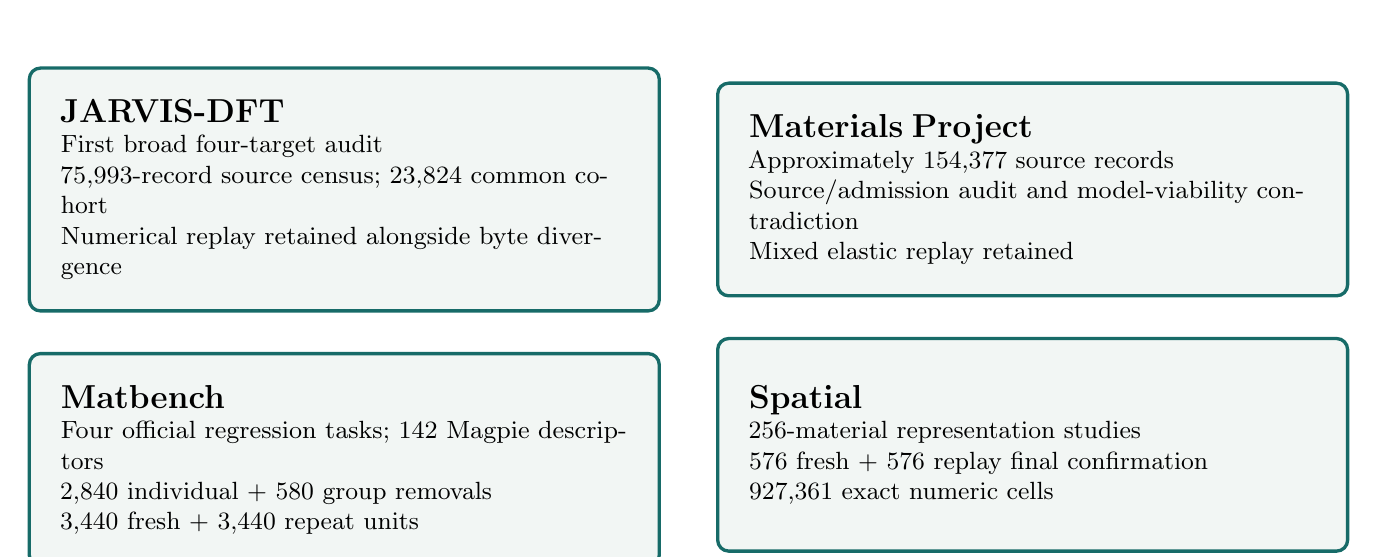
\begin{tikzpicture}[node distance=5mm, every node/.style={font=\small,align=left}, box/.style={draw=teal,very thick,rounded corners,fill=pale,text width=7.2cm,minimum height=2.7cm,inner sep=4mm}]
\node[box] (j) {\textbf{\large JARVIS-DFT}\\First broad four-target audit\\75,993-record source census; 23,824 common cohort\\Numerical replay retained alongside byte divergence};
\node[box,right=7mm of j] (m) {\textbf{\large Materials Project}\\Approximately 154,377 source records\\Source/admission audit and model-viability contradiction\\Mixed elastic replay retained};
\node[box,below=of j] (b) {\textbf{\large Matbench}\\Four official regression tasks; 142 Magpie descriptors\\2,840 individual + 580 group removals\\3,440 fresh + 3,440 repeat units};
\node[box,below=of m] (s) {\textbf{\large Spatial}\\256-material representation studies\\576 fresh + 576 replay final confirmation\\927,361 exact numeric cells};
\end{tikzpicture}

\vspace{7mm}
\begin{tabularx}{\textwidth}{p{0.20\textwidth}Y}
\toprule Route & Principal scientific job\\\midrule
JARVIS & Establish whether compact descriptors carry useful signal across targets, populations, models, scales, and disturbances.\\
Materials Project & Test source suitability and expose disagreement between relative null success and absolute prediction.\\
Matbench & Directly compare fitted permutation importance with complete retrained-removal consequence.\\
Spatial & Test whether structural representation effects persist across larger cohorts, controls, split views, and replay.\\
\bottomrule\end{tabularx}

\vfill
\card{Evidence boundary.}{The source providers performed the underlying first-principles calculations. This programme consumed published records; it did not recompute the providers' DFT corpora locally.}
\newpage

% PAGE 3
\section*{The three headline results}

{\Huge\bfseries\color{gold} 0.0394}\quad {\Large\bfseries Paper 1: fitted use versus retrained dependence}

A descriptor that looked important to the already-trained model was often not the descriptor whose removal mattered most after the network was allowed to retrain.

\begin{itemize}
\item Mean top-10 overlap: 0.100.
\item 3,440 fresh + 3,440 same-environment repeat units; 65,740 numeric cells matched exactly.
\item ``Necessity'' means only retrained-removal consequence in the declared representation, not causal or physical necessity.
\end{itemize}

\vspace{4mm}\hrule\vspace{4mm}
{\Huge\bfseries\color{rust} 73.3\% $\rightarrow$ 4.51\%}\quad {\Large\bfseries Paper 2: signal versus viability}

On the same 288 eligible Materials Project elasticity cells, 73.3\% beat their paired broken-target null, but only 4.51\% achieved positive held-out $R^2$.

\begin{itemize}
\item 13/288 passed both demonstrated gates; all were bulk-modulus cells.
\item $R^2>0$ is only a minimal metric boundary against the evaluated-set constant reference, not practical engineering usefulness.
\end{itemize}

\vspace{4mm}\hrule\vspace{4mm}
{\Large\bfseries\color{blue} Paper 3: evidence state versus engineering permission}

\begin{center}\large\bfseries
AVAILABLE $\rightarrow$ ADMITTED $\rightarrow$ VIABLE $\rightarrow$ REPLAY-ADJUDICATED $\rightarrow$ ACTION-BOUNDED
\end{center}

Each state answers a different question. A stronger downstream claim cannot be inferred merely because an earlier computation succeeded. Exact replay can reproduce a PASS, a failure, or a conditional result.

\vfill
\card{Not claimed.}{No universal descriptor hierarchy, physical mechanism, external replication, engineering qualification, or universal model-acceptance threshold is claimed.}
\newpage

% PAGE 4
\section*{Why it switches from materials ML to engineering}
\begin{center}{\LARGE\bfseries\color{ink} Materials ML showed the evidence problem. Engineering showed why it mattered.}\end{center}

\begin{center}
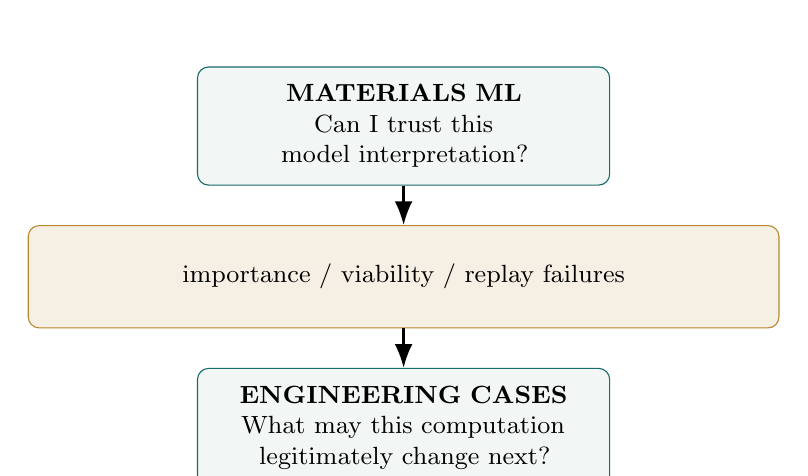
\begin{tikzpicture}[node distance=5mm,every node/.style={align=center,font=\small},box/.style={draw=teal,rounded corners,fill=pale,text width=5.0cm,minimum height=1.5cm},wide/.style={draw=gold,rounded corners,fill=cream,text width=9.3cm,minimum height=1.3cm}]
\node[box] (ml) {\textbf{MATERIALS ML}\\Can I trust this model interpretation?};
\node[wide,below=of ml] (fail) {importance / viability / replay failures};
\node[box,below=of fail] (eng) {\textbf{ENGINEERING CASES}\\What may this computation legitimately change next?};
\draw[-{Latex[length=3mm]},thick] (ml)--(fail);\draw[-{Latex[length=3mm]},thick] (fail)--(eng);
\end{tikzpicture}
\end{center}

\begin{tabularx}{\textwidth}{p{0.16\textwidth}YY}
\toprule Case & Contradiction exposed & Bounded result\\\midrule
Furnace & Corrected geometry broke transfer of an inherited thermal result; cooling added a failure dependency & Guarded coupon, not fabrication\\
Dual tank & State/provenance routes could not be collapsed; invalid return transitions were rejected & Tracer rig, not deployment\\
Heat shield & Segmentation improved containment but degraded thermal performance & Matched coupons, not qualification\\
\bottomrule\end{tabularx}

\stripline{13 candidates $|$ 5 descendants $|$ 116 scenarios $|$ 9,150 uncertainty runs $|$ $\ge$9,380 model operations}

\begin{center}\bfseries
CASE-SPECIFIC WORK $\rightarrow$ RECURRING CONTROL NEEDS $\rightarrow$ LATER SYSTEMICA SERVICES
\end{center}

The cases did not retrospectively run the complete modern architecture. They exposed recurring needs that were later formalised into reusable identity, state, recovery, replay, evidence, memory, and bounded-authority services.
\newpage

% PAGE 5
\section*{How much ran, and what counts as a unit?}
\begin{center}
{\Huge\bfseries\color{gold} 8,836}\par
{\Large committed scientific-unit executions}\\[2mm]
{\large 4,432 primary/fresh $|$ 3,440 same-environment repeat $|$ 964 predecessor-linked replay}
\end{center}

\card{Scientific unit.}{The smallest contract-bound part of an experiment allowed to complete independently after required outputs, schemas, and identity checks pass. A unit is not a fixed amount of compute.}

\begin{tabularx}{\textwidth}{p{0.20\textwidth}YY}
\toprule Example & Unit anatomy & Why the distinction matters\\\midrule
Matbench V0.2 & 20 official-fold units; each held one baseline + five null fits & 20 units represented 120 estimator fits\\
Matbench V0.3 & 3,440 task--fold--operation units per identity & Included 2,840 individual and 580 group-removal refits\\
Spatial V0.6.1 & 144 valid + 432 paired-null units per identity & 576 units represented a labelled confirmation plan, not 576 rows\\
\bottomrule\end{tabularx}

\stripline{$\ge$1,059,273 NUMERIC FRESH$\leftrightarrow$REPEAT/REPLAY CELLS COMPARED}

That comparison count is not the number of calculations. Source scale is also separate: approximately 230,370 provenance-separated JARVIS + Materials Project records were touched. Matbench contributes 260,839 task-record instances, not unique materials and not an additive source census.

\begin{center}\small\ttfamily
[RUN] -- [ordinary use/review] -- [INTERRUPT/CHECKPOINT] -- [RESUME] -- [REPLAY]
\end{center}

The shared workstation did not run as one continuous benchmark campaign. Calendar gaps include ordinary use and review. Scientific identity followed verified committed work. JARVIS and Materials Project both exercised real resume behaviour; incomplete staging was not accepted.

\begin{center}\bfseries Resume is not replication. Replay is not automatically external replication.\end{center}
\newpage

% PAGE 6
\section*{Worked translation: from computation to bounded action}
\begin{center}
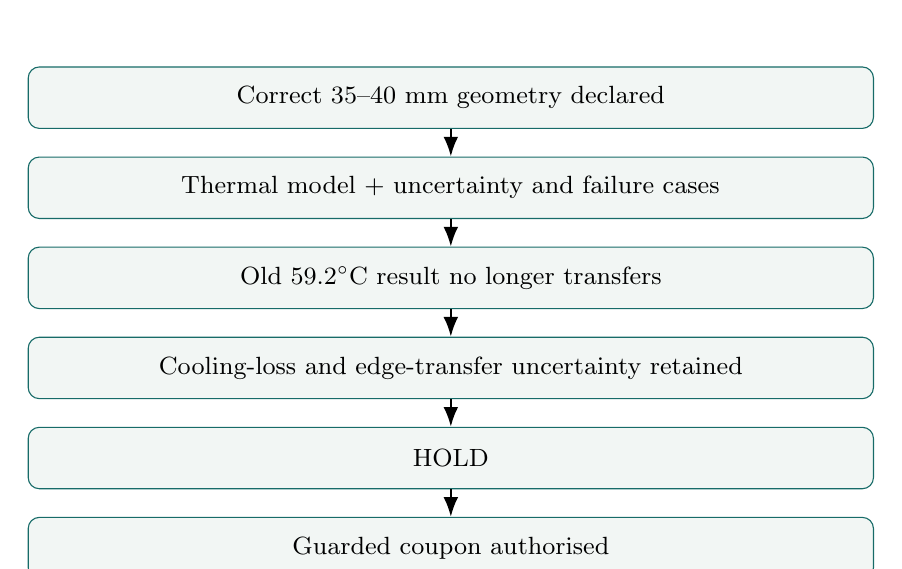
\begin{tikzpicture}[node distance=3.5mm,every node/.style={font=\small,align=center},stage/.style={draw=teal,rounded corners,fill=pale,text width=10.5cm,minimum height=0.78cm}]
\node[stage] (a) {Correct 35--40 mm geometry declared};
\node[stage,below=of a] (b) {Thermal model + uncertainty and failure cases};
\node[stage,below=of b] (c) {Old 59.2$^\circ$C result no longer transfers};
\node[stage,below=of c] (d) {Cooling-loss and edge-transfer uncertainty retained};
\node[stage,below=of d] (e) {HOLD};
\node[stage,below=of e] (f) {Guarded coupon authorised};
\foreach \x/\y in {a/b,b/c,c/d,d/e,e/f}{\draw[-{Latex[length=2.5mm]},thick] (\x)--(\y);}
\end{tikzpicture}
\end{center}

\textbf{Translate it to your workflow.} What exact object/configuration is being judged? Which predecessor evidence still belongs to it? Which failures must remain visible? What would make it ineligible to progress? What is the smallest next action the evidence earns?

\begin{center}\small\bfseries
EXECUTION $\rightarrow$ COMPARISON $\rightarrow$ CANDIDATE CLAIM $\rightarrow$ HUMAN DECISION $\rightarrow$ BOUNDED UPDATE OR HOLD
\end{center}
An unconfirmed eligible claim was refused with zero writes. Explicit human review accepted bounded Matbench and Spatial-bulk claims with exact read-back, while attempted upgrades of Spatial shear and Materials Project elasticity were refused. No engineering action was created.

\begin{tabularx}{\textwidth}{p{0.47\textwidth}p{0.47\textwidth}}
\toprule Question & Short answer\\\midrule
Isn't Paper 1 obvious? & The distinction is known; the contribution is measuring its size and structure under a frozen materials protocol.\\
Isn't Paper 2 just algebra? & The inequality is trivial; the empirical 211/288 versus 13/288 disagreement is not.\\
Does $R^2>0$ mean useful? & No. It is only a minimal metric boundary.\\
Does exact replay prove truth? & No. Replay can exactly reproduce a failed or conditional result.\\
Why not publish the whole runtime? & Claim-bearing evidence and exact method specifications are public; reusable orchestration and commercial implementation remain private pending IP review.\\
Do the cases prove universal Systemica validity? & No. They provide local control-transfer evidence, not industrial or universal validation.\\
Was this generated by AI? & AI/coding tools assisted development and drafting; frozen analyses ran through declared scientific software and conclusions were reviewed by the author.\\
Is it peer reviewed? & Not yet. These are public preprints and an inspectable evidence programme.\\
Can someone reproduce everything? & Principal claims can be reconstructed publicly; independent clean-room re-execution remains a stronger future replication level.\\
\bottomrule\end{tabularx}

\vspace{2mm}
\begin{center}{\large\bfseries\color{ink} If you remember one thing: ask what the evidence actually tested before allowing it to justify the next claim or action.}\end{center}

\end{document}
